\documentclass{article}
\usepackage{amsmath}
\usepackage{amssymb}
\usepackage{graphicx}
\usepackage{tikz}
\usepackage{url}
\usepackage{circuitikz}
%\usetikzlibrary{circuits.ee.IEC}
\usetikzlibrary{shapes,arrows}
\usepackage{circuitikz}

\title{\textbf{Lab Report: Experiment 6}}
\author{EE24BTECH11003 : Akshara Sarma Chennubhatla\\EE24BTECH11005 : Arjun Pavanje}

\begin{document}
\maketitle
\begin{center}
	\textbf{Experiment:} Design, implementation, and analysis\\of a bandpass filter constructed by\\cascading Sallen-Key second-order\\low-pass and high-pass filters.\\Analysis of Bode plots of HPF, LPF and BPF.
\end{center}
\vspace{30pt}
\begin{figure}[h!]
	\centering
	
\includegraphics[width = 100pt]{.logo/logo.png}\\
\end{figure}
\begin{center}
	Bachelor of Technology\\
	\vspace{10pt}
	Department of Electrical Engineering\\
\end{center}
\newpage

\section*{1 Introduction}

This experiment focuses on implementing a bandpass filter using the Sallen-Key topology, a versatile active filter design that employs operational amplifiers.

The bandpass filter is constructed by cascading a high-pass filter (HPF) and a low-pass filter (LPF). The HPF attenuates frequencies below its cutoff frequency ($\omega_{c1}$), while the LPF attenuates frequencies above its cutoff frequency ($\omega_{c2}$). When properly designed with $\omega_{c2} > \omega_{c1}$, the combined response creates a bandpass characteristic.

The Sallen-Key topology offers a simple, low-component design with high input impedance and low output impedance, making it ideal for active filters with minimal component interaction and predictable performance.

\section*{Sallen Key Filter Circuit}

\begin{figure}[!ht]
\centering
\resizebox{0.8\textwidth}{!}{%
\begin{circuitikz}
\tikzstyle{every node}=[font=\LARGE]
\draw (12.75,10.75) node[op amp,scale=1, yscale=-1 ] (opamp2) {};
\draw (opamp2.+) to[short] (11.25,11.25);
\draw  (opamp2.-) to[short] (11.25,10.25);
\draw (13.95,10.75) to[short](14.25,10.75);
\draw (11.25,10.25) to[short] (11.25,9);
\draw (11.25,9) to[short] (14,9);
\draw (14,9) to[short] (14,10.75);
\draw (14.25,10.75) to[short] (14.75,10.75);
\draw (11.25,11.25) to[short] (10.5,11.25);
\draw (10.5,11.25) to[european resistor] (10.5,8.75);
\draw (7,11.25) to[european resistor] (8.75,11.25);
\draw (8.75,11.25) to[european resistor] (10.5,11.25);
\draw (8.75,11.25) to[short] (8.75,13.25);
\draw (8.75,13.25) to[european resistor] (13.5,13.25);
\draw (13.5,13.25) to[short] (13.5,10.75);
\draw (7,11.25) to[short] (6.5,11.25);
\node at (8.75,11.25) [circ] {};
\node at (10.5,11.25) [circ] {};
\node at (14,10.75) [circ] {};
\node at (13.5,10.75) [circ] {};
\node at (14.75,10.75) [circ] {};
\node at (6.5,11.25) [circ] {};
\node [font=\normalsize] at (6,11.25) {$V_{in}$};
\node [font=\normalsize] at (15.25,10.75) {$V_{out}$};
\node [font=\normalsize] at (7.75,10.75) {$Z_1$};
\node [font=\normalsize] at (9.5,10.75) {$Z_2$};
\node [font=\normalsize] at (10,10) {$Z_3$};
\node [font=\normalsize] at (11,13.75) {$Z_4$};
\node [font=\normalsize] at (8.75,11) {a};
\node [font=\normalsize] at (10.75,11) {b};
\draw (10.5,8.75) to (10.75,8.75) node[ground]{};
\end{circuitikz}
}%
\end{figure}

\subsection*{Derivation of Transfer function for Sallen Key Filter:\\}
For ideal Op Amp,
\begin{align*}
V_b = V_{out}
\end{align*}
Applying KCL at a:
\begin{align*}
\frac{V_a - V_{in}}{Z_1} + \frac{V_a-V_b}{Z_2} + \frac{V_a-V_{out}}{Z_4} &= 0 \quad \text{-(1)}
\end{align*}
Applyting KCL at b:
\begin{align*}
\frac{V_b-V_a}{Z_2} + \frac{V_b-0}{Z_3} &= 0 \\
V_b\left(\frac{1}{Z_2} + \frac{1}{Z_3}\right) &= \frac{V_a}{Z_2} \\
V_a &= V_b Z_2\left(\frac{1}{Z_2} + \frac{1}{Z_3}\right)
\end{align*}
Simplifying (1)
\begin{align*}
V_a\left(\frac{1}{Z_1} + \frac{1}{Z_2} + \frac{1}{Z_4}\right) - \frac{V_{in}}{Z_1} &= V_{out}\left(\frac{1}{Z_2} + \frac{1}{Z_4}\right) \\
V_{out} Z_2\left(\frac{1}{Z_2} + \frac{1}{Z_3}\right)\left(\frac{1}{Z_1} + \frac{1}{Z_2} + \frac{1}{Z_4}\right) - \frac{V_{in}}{Z_1} &= V_{out}\left(\frac{1}{Z_2} + \frac{1}{Z_4}\right) 
\end{align*}
\begin{align*}
H(s) &= \frac{V_{out}}{V_{in}} = \frac{\frac{1}{Z_1}}{Z_2\left(\frac{1}{Z_2} + \frac{1}{Z_3}\right)\left(\frac{1}{Z_1} + \frac{1}{Z_2} + \frac{1}{Z_4}\right) - \left(\frac{1}{Z_2} + \frac{1}{Z_4}\right)} \\
H(s) &= \frac{\frac{1}{Z_1}}{\frac{(Z_2+Z_3)(Z_1Z_2+Z_1Z_4+Z_2Z_4) - (Z_2+Z_4)Z_1Z_3}{Z_1Z_2Z_3Z_4}} \\
 &= \frac{Z_2Z_3Z_4}{(Z_2+Z_3)(Z_1Z_2+Z_1Z_4+Z_2Z_4) - Z_1Z_3(Z_2+Z_4)} \\
 &= \frac{Z_3Z_4}{Z_1Z_2^2 + Z_1Z_2Z_4 + Z_2^2Z_4 + Z_1Z_3Z_4} \\
 &= \frac{Z_3Z_4}{Z_1Z_2 + Z_1Z_4 + Z_2Z_4 + Z_3Z_4}
\end{align*}

\section*{Theory}

\subsection*{Bandpass Filter Principle}

A bandpass filter allows signals within a specific frequency band to pass while attenuating signals outside this band. The transfer function of an ideal bandpass filter can be expressed as:

\[
H(j\omega) = 
\begin{cases}
1, & \text{if } \omega_1 < \omega < \omega_2 \\
0, & \text{otherwise}
\end{cases}
\]

Where $\omega_1 = 2\pi f_{c1}$ and $\omega_2 = 2\pi f_{c2}$ represent the lower and upper cutoff frequencies, respectively.

\subsection*{Sallen-Key Filter Topology}

The Sallen-Key topology is a versatile active filter configuration that uses an operational amplifier with RC components to create second-order filter responses. The general transfer function of a second-order Sallen-Key filter is:

\[
H(s) = \frac{A}{s^2 + (\omega_c/Q)s + \omega_c^2}
\]

Where:
\begin{itemize}
\item $\omega_c$ is the cutoff frequency
\item $Q$ is the quality factor
\item $A$ is the gain at passband
\end{itemize}

\subsubsection*{Sallen-Key Low-Pass Filter}

\begin{figure}[!ht]
\centering
\resizebox{0.8\textwidth}{!}{%
\begin{circuitikz}
\tikzstyle{every node}=[font=\LARGE]
\draw (12.75,10.75) node[op amp,scale=1, yscale=-1 ] (opamp2) {};
\draw (opamp2.+) to[short] (11.25,11.25);
\draw  (opamp2.-) to[short] (11.25,10.25);
\draw (13.95,10.75) to[short](14.25,10.75);
\draw (11.25,10.25) to[short] (11.25,9);
\draw (11.25,9) to[short] (14,9);
\draw (14,9) to[short] (14,10.75);
\draw (14.25,10.75) to[short] (14.75,10.75);
\draw (11.25,11.25) to[short] (10.5,11.25);
%\draw (10.5,11.25) to[european resistor] (10.5,8.75);
\draw (10.5, 11.25) to[C] (10.5, 8.75);
\draw (7,11.25) to[R] (8.75,11.25);
\draw (8.75,11.25) to[R] (10.5,11.25);
\draw (8.75,11.25) to[short] (8.75,13.25);
\draw (8.75,13.25) to[C] (13.5,13.25);
\draw (13.5,13.25) to[short] (13.5,10.75);
\draw (7,11.25) to[short] (6.5,11.25);
\node at (8.75,11.25) [circ] {};
\node at (10.5,11.25) [circ] {};
\node at (14,10.75) [circ] {};
\node at (13.5,10.75) [circ] {};
\node at (14.75,10.75) [circ] {};
\node at (6.5,11.25) [circ] {};
\node [font=\normalsize] at (6,11.25) {$V_{in}$};
\node [font=\normalsize] at (15.25,10.75) {$V_{out}$};
\node [font=\normalsize] at (7.75,10.75) {$R$};
\node [font=\normalsize] at (9.5,10.75) {$R$};
\node [font=\normalsize] at (9.75,10) {$C$};
\node [font=\normalsize] at (11,14) {$C$};
\node [font=\normalsize] at (8.75,11) {a};
\node [font=\normalsize] at (10.75,11) {b};
\draw (10.5,8.75) to (10.75,8.75) node[ground]{};
\end{circuitikz}
}%
\end{figure}

\begin{align*}
Z_1 &= Z_2 = R_1\\
Z_3 &= Z_4 = \frac{1}{SC_1}\\
H(s) &= \frac{\left(\frac{1}{SC_1}\right)^2}{R_1^2 + \frac{2R_1}{SC_1} + (\frac{1}{SC_1})^2}\\
H(s) &= \frac{1}{(1 + SR_1C_1)^2}
\end{align*}

The cutoff frequency for the Sallen-Key LPF is given by:

\[
\omega_{c_1} = \frac{1}{R_1C_1}
\]

\pagebreak
\subsubsection*{Sallen-Key High-Pass Filter}

\begin{figure}[!ht]
\centering
\resizebox{1\textwidth}{!}{%
\begin{circuitikz}
\tikzstyle{every node}=[font=\LARGE]
\draw (12.75,10.75) node[op amp,scale=1, yscale=-1 ] (opamp2) {};
\draw (opamp2.+) to[short] (11.25,11.25);
\draw  (opamp2.-) to[short] (11.25,10.25);
\draw (13.95,10.75) to[short](14.25,10.75);
\draw (11.25,10.25) to[short] (11.25,9);
\draw (11.25,9) to[short] (14,9);
\draw (14,9) to[short] (14,10.75);
\draw (14.25,10.75) to[short] (14.75,10.75);
\draw (11.25,11.25) to[short] (10.5,11.25);
%\draw (10.5,11.25) to[european resistor] (10.5,8.75);
\draw (10.5, 11.25) to[R] (10.5, 8.75);
\draw (7,11.25) to[C] (8.75,11.25);
\draw (8.75,11.25) to[C] (10.5,11.25);
\draw (8.75,11.25) to[short] (8.75,13.25);
\draw (8.75,13.25) to[R] (13.5,13.25);
\draw (13.5,13.25) to[short] (13.5,10.75);
\draw (7,11.25) to[short] (6.5,11.25);
\node at (8.75,11.25) [circ] {};
\node at (10.5,11.25) [circ] {};
\node at (14,10.75) [circ] {};
\node at (13.5,10.75) [circ] {};
\node at (14.75,10.75) [circ] {};
\node at (6.5,11.25) [circ] {};
\node [font=\normalsize] at (6,11.25) {$V_{in}$};
\node [font=\normalsize] at (15.25,10.75) {$V_{out}$};
\node [font=\normalsize] at (7.75,10.5) {$C$};
\node [font=\normalsize] at (9.5,10.5) {$C$};
\node [font=\normalsize] at (10,10) {$R$};
\node [font=\normalsize] at (11,13.75) {$R$};
\node [font=\normalsize] at (8.75,11) {a};
\node [font=\normalsize] at (10.75,11) {b};
\draw (10.5,8.75) to (10.75,8.75) node[ground]{};
\end{circuitikz}
}%
\end{figure}
\begin{align*}
Z_1 &= Z_2 = \frac{1}{SC_2}\\
Z_3 &= Z_4 = R_2\\
H(s) &= \frac{R_2^2}{R_2^2 + \frac{2R_2}{SC_2} + (\frac{1}{SC_2})^2}\\
H(s) &= \frac{{(SR_2C_2)}^2}{(1 + SR_2C_2)^2}
\end{align*}

The cutoff frequency for the Sallen-Key LPF is given by:

\[
\omega_{c_2} = \frac{1}{R_2C_2}
\]

\pagebreak
\subsection*{Cascaded Bandpass Filter}

\begin{figure}[!ht]
\centering
\resizebox{1\textwidth}{!}{%
\begin{circuitikz}
\tikzstyle{every node}=[font=\normalsize]
\draw (3.75,13) to[R,l={ \normalsize R}] (6.25,13);
\draw (4.5,13) to[short, -o] (3.75,13) ;
\draw (6.25,13) to[short] (6.25,14.25);
\draw (6.25,13) to[R,l={ \normalsize R}] (8,13);
\draw (10.25,12.5) node[op amp,scale=1, yscale=-1 ] (opamp2) {};
\draw (opamp2.+) to[short] (8.75,13);
\draw  (opamp2.-) to[short] (8.75,12);
\draw (11.45,12.5) to[short](11.75,12.5);
\draw (8,13) to[C,l={ \normalsize C}] (8,10.5);
\draw (8,13) to[short] (8.75,13);
\draw (6.25,14.25) to[C,l={ \normalsize C}] (11.75,14.25);
\draw (11.75,14.25) to[short] (11.75,10.5);
\draw (11.75,12.5) to[C,l={ \normalsize C}] (13.75,12.5);
\draw (13.75,12.5) to[C,l={ \normalsize C}] (16.25,12.5);
\draw (17.75,12) node[op amp,scale=1, yscale=-1 ] (opamp2) {};
\draw (opamp2.+) to[short] (16.25,12.5);
\draw  (opamp2.-) to[short] (16.25,11.5);
\draw (18.95,12) to[short](19.25,12);
\draw (15.75,12.5) to[R,l={ \normalsize R}] (15.75,9.5);
\draw (13.75,14.25) to[R,l={ \normalsize R}] (19.25,14.25);
\draw (13.75,12.5) to[short] (13.75,14.25);
\draw (16.25,11.5) to[short] (16.25,9.25);
\draw (16.25,9.25) to[short] (19.25,9.25);
\draw (19.25,9.25) to[short] (19.25,14.25);
\draw (19.25,12) to[short, -o] (20,12) ;
\draw (15.75,10.25) to (15.75,9.25) node[ground]{};
\draw (8,11.25) to (8,10.25) node[ground]{};
\draw (8.75,12) to[short] (8.75,10.5);
\draw (8.75,10.5) to[short] (11.75,10.5);
\draw (17.75,12) node[op amp,scale=1, yscale=-1 ] (opamp2) {};
\draw (opamp2.+) to[short] (16.25,12.5);
\draw  (opamp2.-) to[short] (16.25,11.5);
\draw (18.95,12) to[short](19.25,12);
\end{circuitikz}
}%

\label{fig:my_label}
\end{figure}

When an HPF with cutoff frequency $\omega_{c1}$ is cascaded with an LPF with cutoff frequency $\omega_{c2}$ (where $\omega_{c2} > \omega_{c1}$), the resulting system functions as a bandpass filter with:

\begin{itemize}
\item Lower cutoff frequency: $\omega_{c1}$
\item Upper cutoff frequency: $\omega_{c2}$
\item Bandwidth: $BW = \omega_{c2} - \omega_{c1}$
\item Center frequency: $\omega_0 = \sqrt{\omega_{c1}\omega_{c2}}$
\end{itemize}

The overall transfer function becomes the product of the individual transfer functions:

\[
H_{BPF}(s) = H_{HPF}(s) \cdot H_{LPF}(s)
\]
\begin{align*}
    H_{BPF}(s) = \frac{{(SR_1C_1)}^2}{(1 + SR_1C_1)^2(1 + SR_2C_2)^2}
\end{align*}

\section*{Procedure}

\subsection*{Components}

For this experiment, we select the following components:
\begin{itemize}
\item Operational Amplifier: LM358 (or equivalent)
\item Resistors: $R_1 = R_2 = 1k\Omega$ (for LPF),  $R_3 = R_4 = 15k\Omega$ (for HPF)
\item Capacitors: $C_1 = C_2 = 1nF$ (for LPF), $C_3 = C_4 = 1nF$ (for HPF)
\end{itemize}

The theoretical cutoff frequencies are:
\begin{itemize}
\item HPF: $\omega_{c1} = \frac{1}{(\sqrt{R_1R_2C_1C_2})} = \frac{10^6}{15}$ 
\item LPF: $\omega_{c2} = \frac{1}{(\sqrt{R_3R_4C_3C_4})} = 10^6$
\end{itemize}

\subsection*{High-Pass Filter Implementation}

\begin{enumerate}
\item Assemble the Sallen-Key HPF circuit on the breadboard according to the circuit diagram.
\begin{figure}[h!]
    \centering
    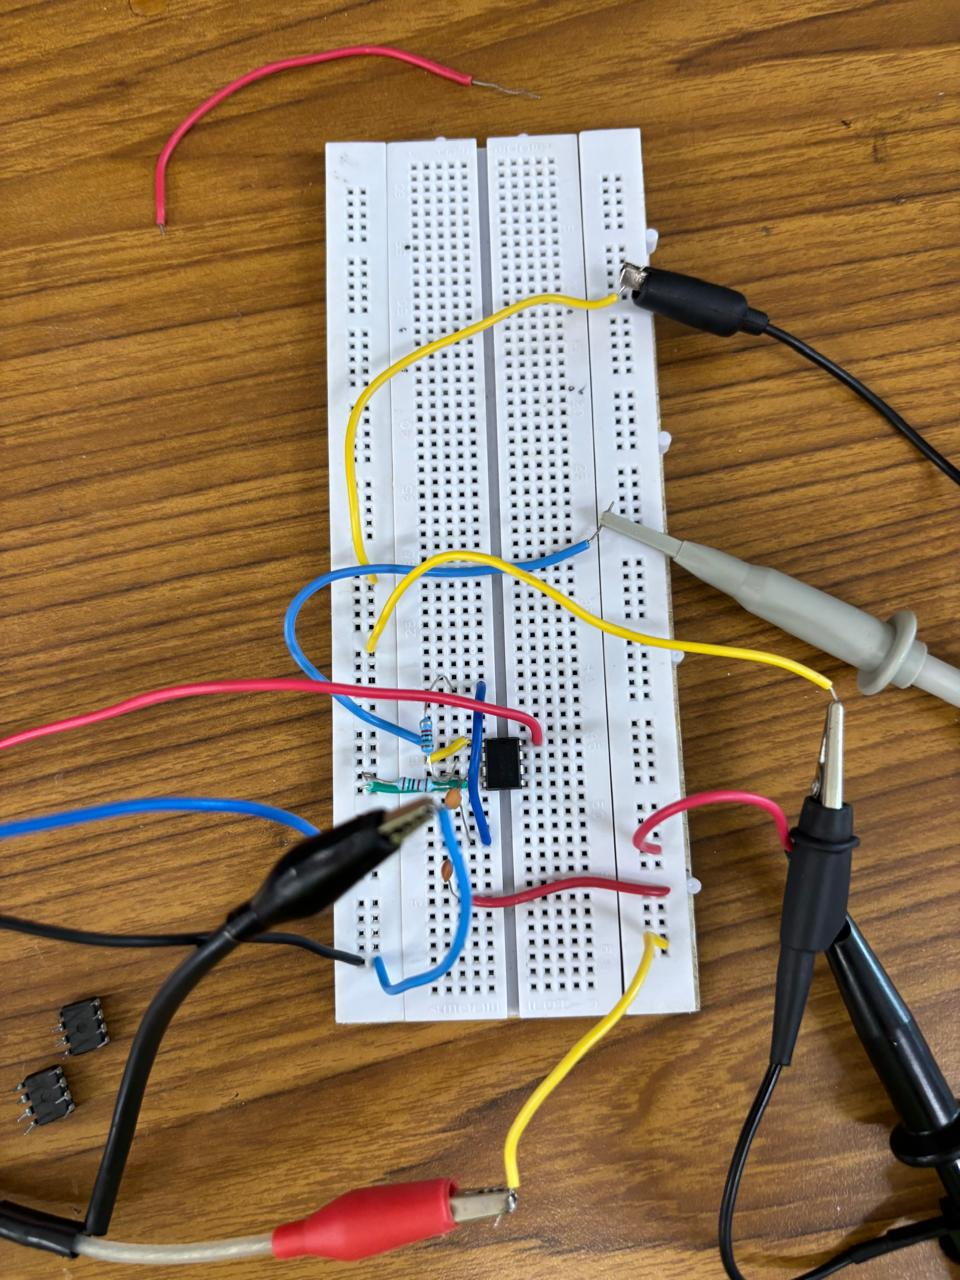
\includegraphics[width=0.5\linewidth]{figs/highpass_ciruit.jpeg}
    \caption{High Pass Filter circuit}
    \label{fig:enter-label}
\end{figure}
\item Connect the function generator to provide a sine wave input.
\item Connect the oscilloscope to measure both input and output signals.
\item Vary the input frequency by atleast doubling each time.
\item For each frequency, measure the output voltage and calculate the gain ($V_{out}/V_{in}$).
\item Record the measurements in a table and plot the bode plot.
\end{enumerate}

\subsection*{4.3 Low-Pass Filter Implementation}

\begin{enumerate}
\item Assemble the Sallen-Key LPF circuit on the breadboard as shown.
\begin{figure}[h!]
    \centering
    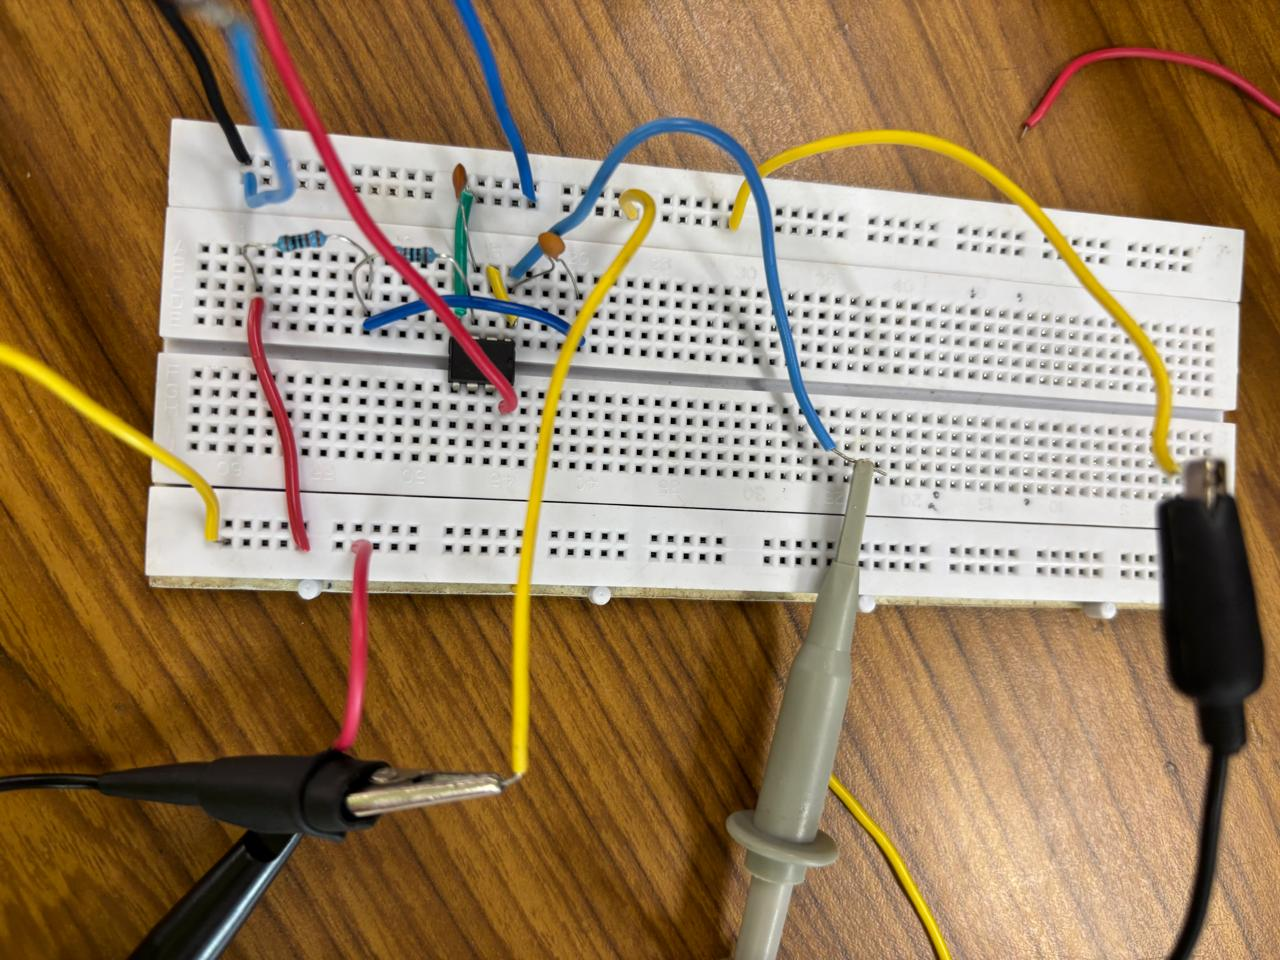
\includegraphics[width=0.7\linewidth]{figs/lowpass_circuit.jpeg}
    \caption{High Pass Filter circuit}
    \label{fig:enter-label}
\end{figure}
\pagebreak
\item Repeat the measurement procedure as in the HPF implementation.
\item Record the measurements and plot the bode plot.
\end{enumerate}

\subsection*{4.4 Bandpass Filter Implementation}

\begin{enumerate}
\item Connect the output of the HPF to the input of the LPF to form the bandpass filter.
\begin{figure}[h!]
    \centering
    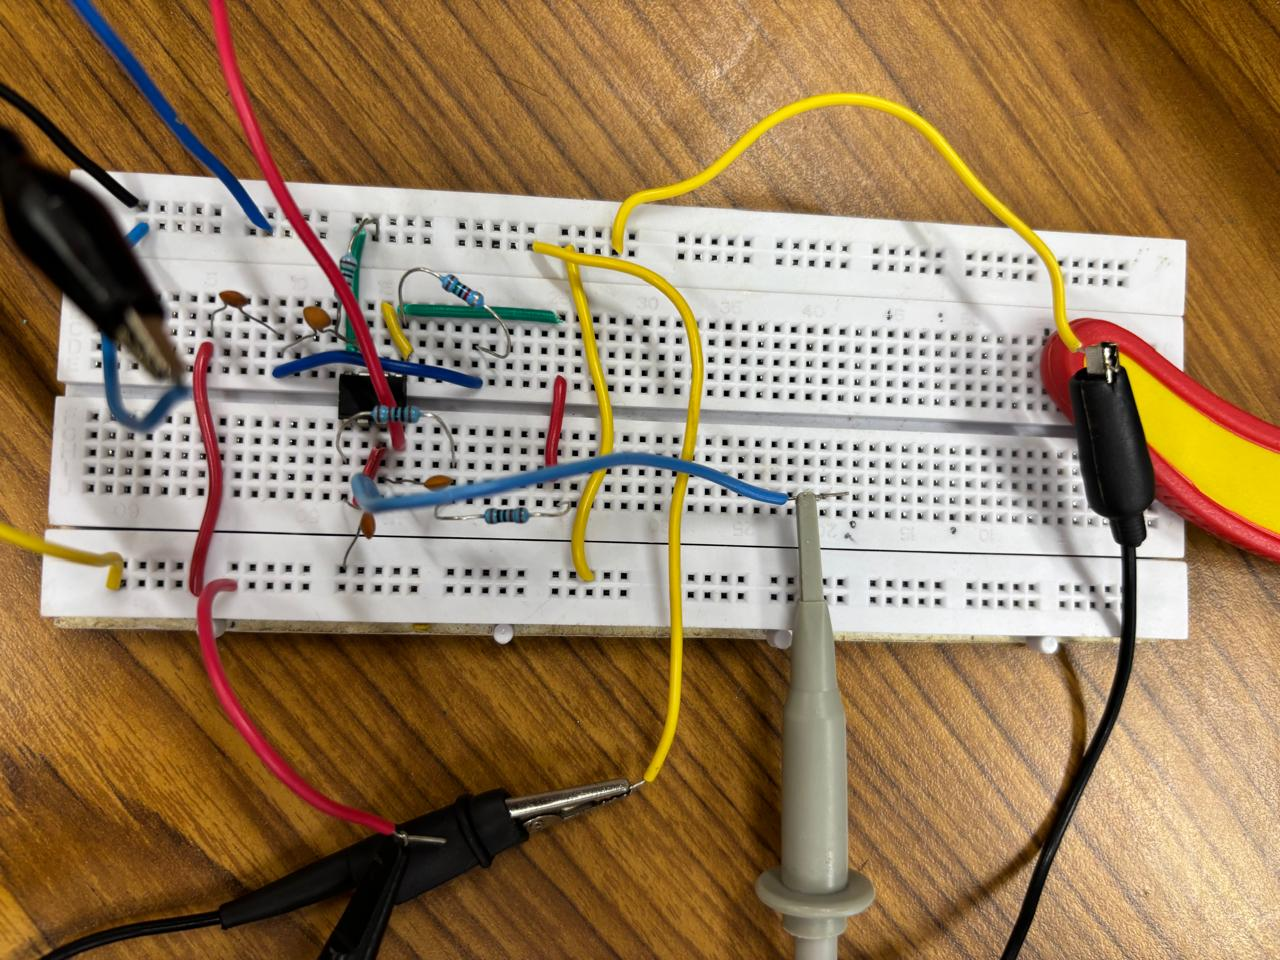
\includegraphics[width=0.7\linewidth]{figs/bandpass_circuit.jpeg}
    \caption{High Pass Filter circuit}
    \label{fig:enter-label}
\end{figure}
\pagebreak
\item Repeat the measurement procedure across the frequency range.
\item Record the measurements and plot the bode plot.
\end{enumerate}

\section*{5 Results and Observations}

Low Pass,
\begin{table}[h!]
\centering
\begin{tabular}{|c|c|}
\hline
$\mathbf{\log{\omega}}$ & $\mathbf{20\log{H(j\omega)}}$ \\
\hline
2.50 & 0.00 \\
2.80 & 0.00 \\
3.10 & 0.00 \\
3.50 & 0.00 \\
3.97 & 0.00 \\
4.50 & 0.00 \\
5.10 & 0.00 \\
5.40 & 0.00 \\
5.70 & -6.38 \\
6.10 & -13.98 \\
6.50 & -27.96 \\
\hline
\end{tabular}
\caption{Low pass filter}
\end{table}
\begin{figure}[h!]
    \centering
    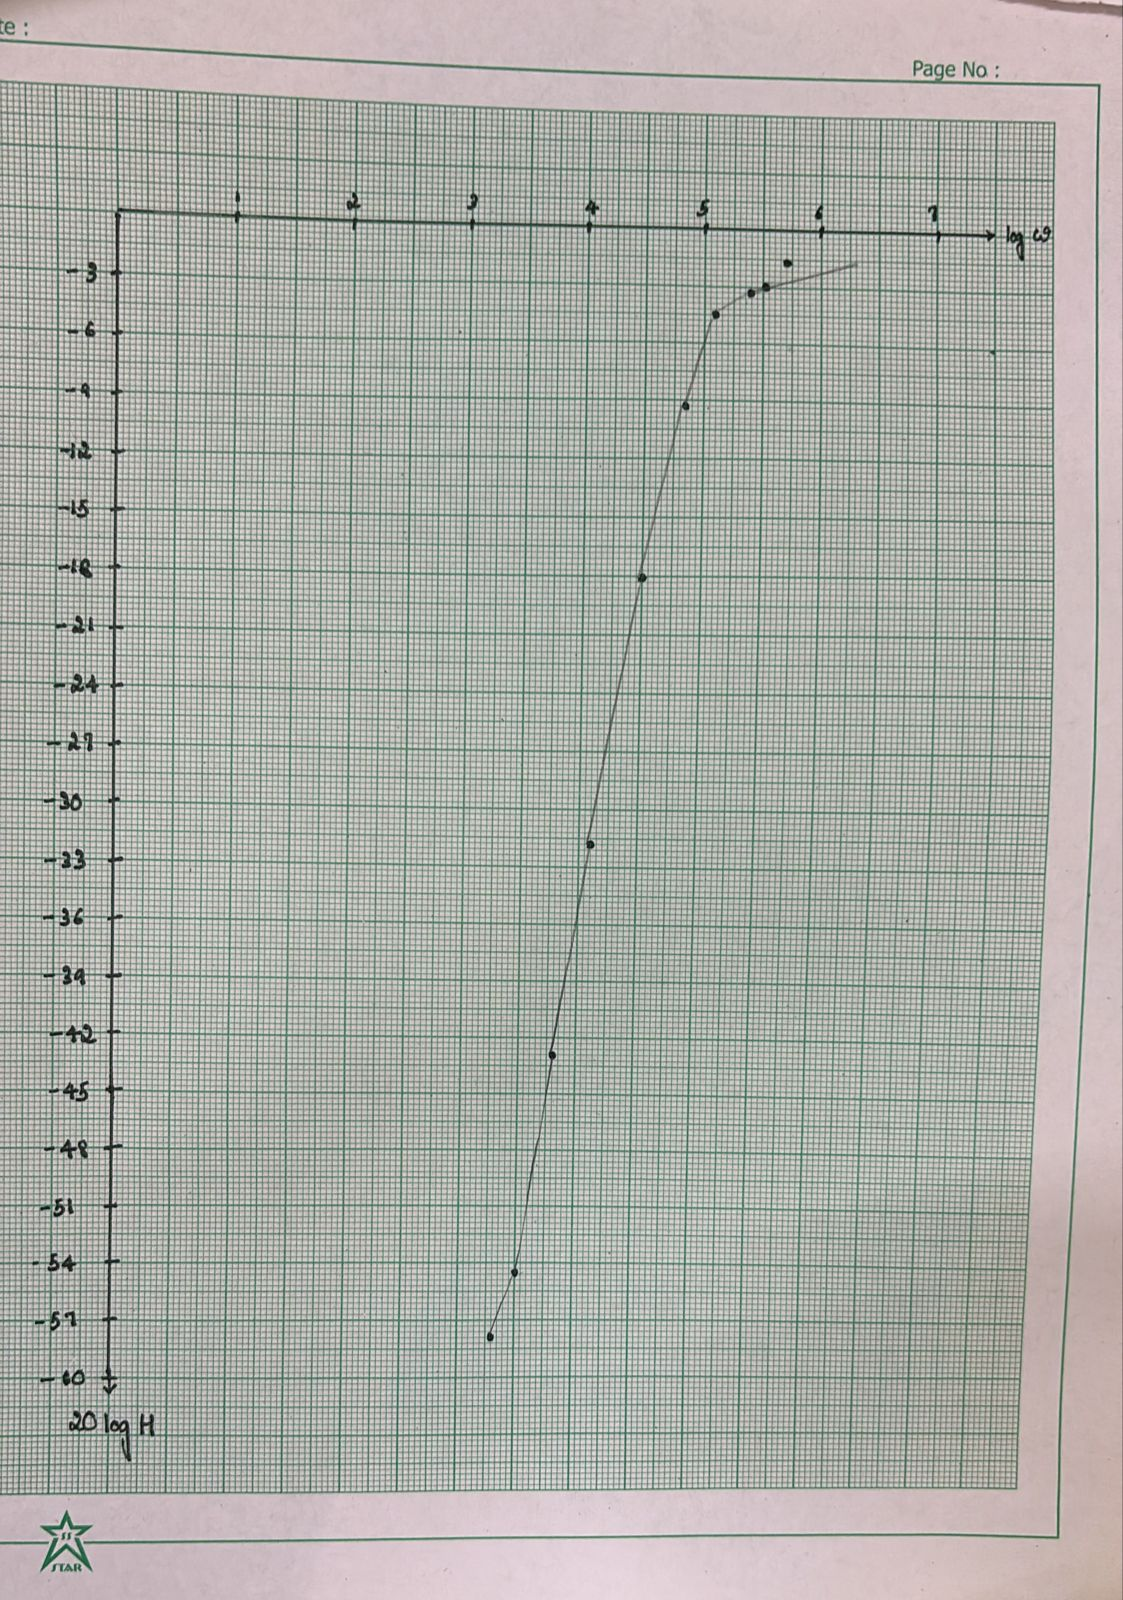
\includegraphics[width=0.5\linewidth]{figs/lowpass_graph.jpeg}
    \caption{Low Pass Filter Graph}
    \label{fig:enter-label}
\end{figure}
HighPass,
\begin{table}[h!]
\centering
\begin{tabular}{|c|c|}
\hline
$\mathbf{\log{\omega}}$ & $\mathbf{20\log{H}}$ \\
\hline
3.28 & -58.06 \\
3.50 & -54.62 \\
3.80 & -42.92 \\
4.10 & -31.93 \\
4.50 & -18.06 \\
4.80 & -9.28 \\
5.10 & -4.53 \\
5.40 & -3.25 \\
5.50 & -2.87 \\
5.70 & -1.58 \\
\hline
\end{tabular}
\caption{High pass filter}
\end{table}
\begin{figure}[h!]
    \centering
    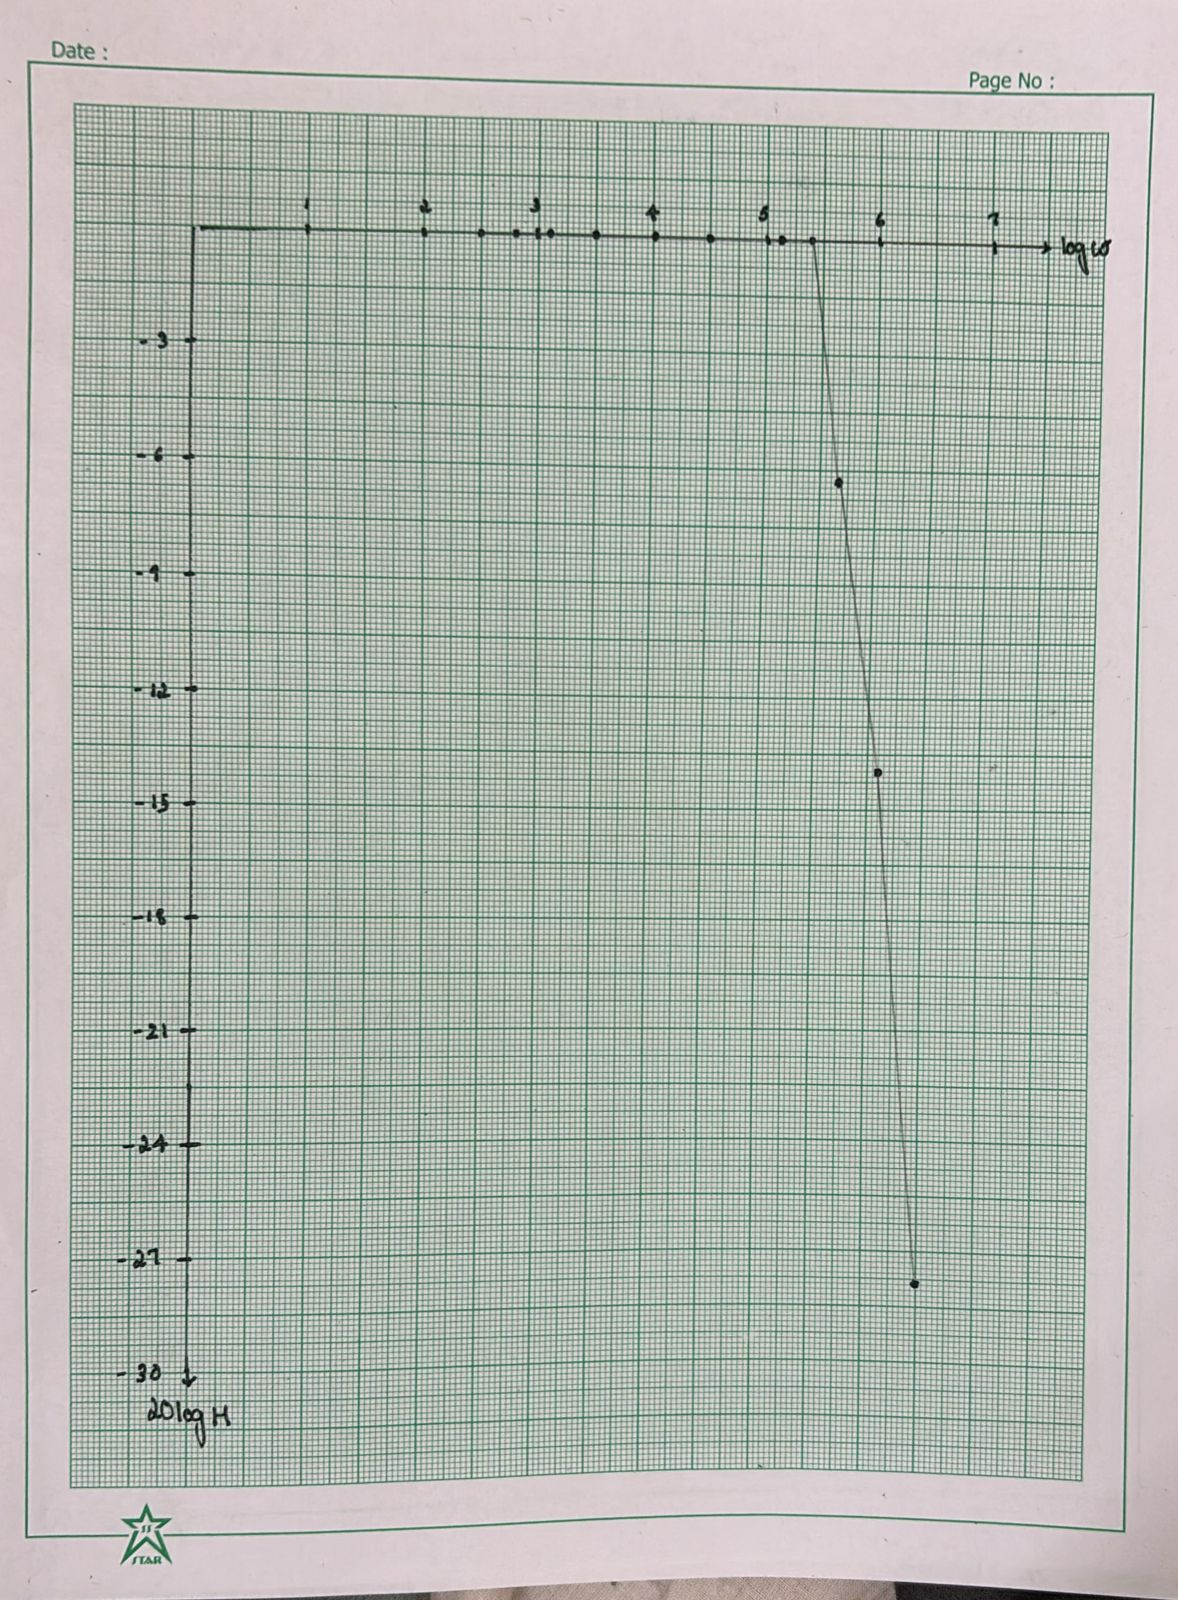
\includegraphics[width=0.5\linewidth]{figs/highpass_graph.jpeg}
    \caption{High Pass Filter Graph}
    \label{fig:enter-label}
\end{figure}


BandPass,
\begin{table}[h!]
\centering
\begin{tabular}{|c|c|}
\hline
$\mathbf{\log{\omega}}$ & $\mathbf{20\log{H}}$ \\
\hline
4.50 & -20.67 \\
4.80 & -9.90 \\
4.97 & -5.85 \\
5.28 & -3.44 \\
5.50 & -3.44 \\
5.80 & -5.69 \\
6.10 & -15.88 \\
6.20 & -20.98 \\
\hline
\end{tabular}
\caption{Band pass filter}
\label{tab:w_vs_H}
\end{table}
\begin{figure}[h!]
    \centering
    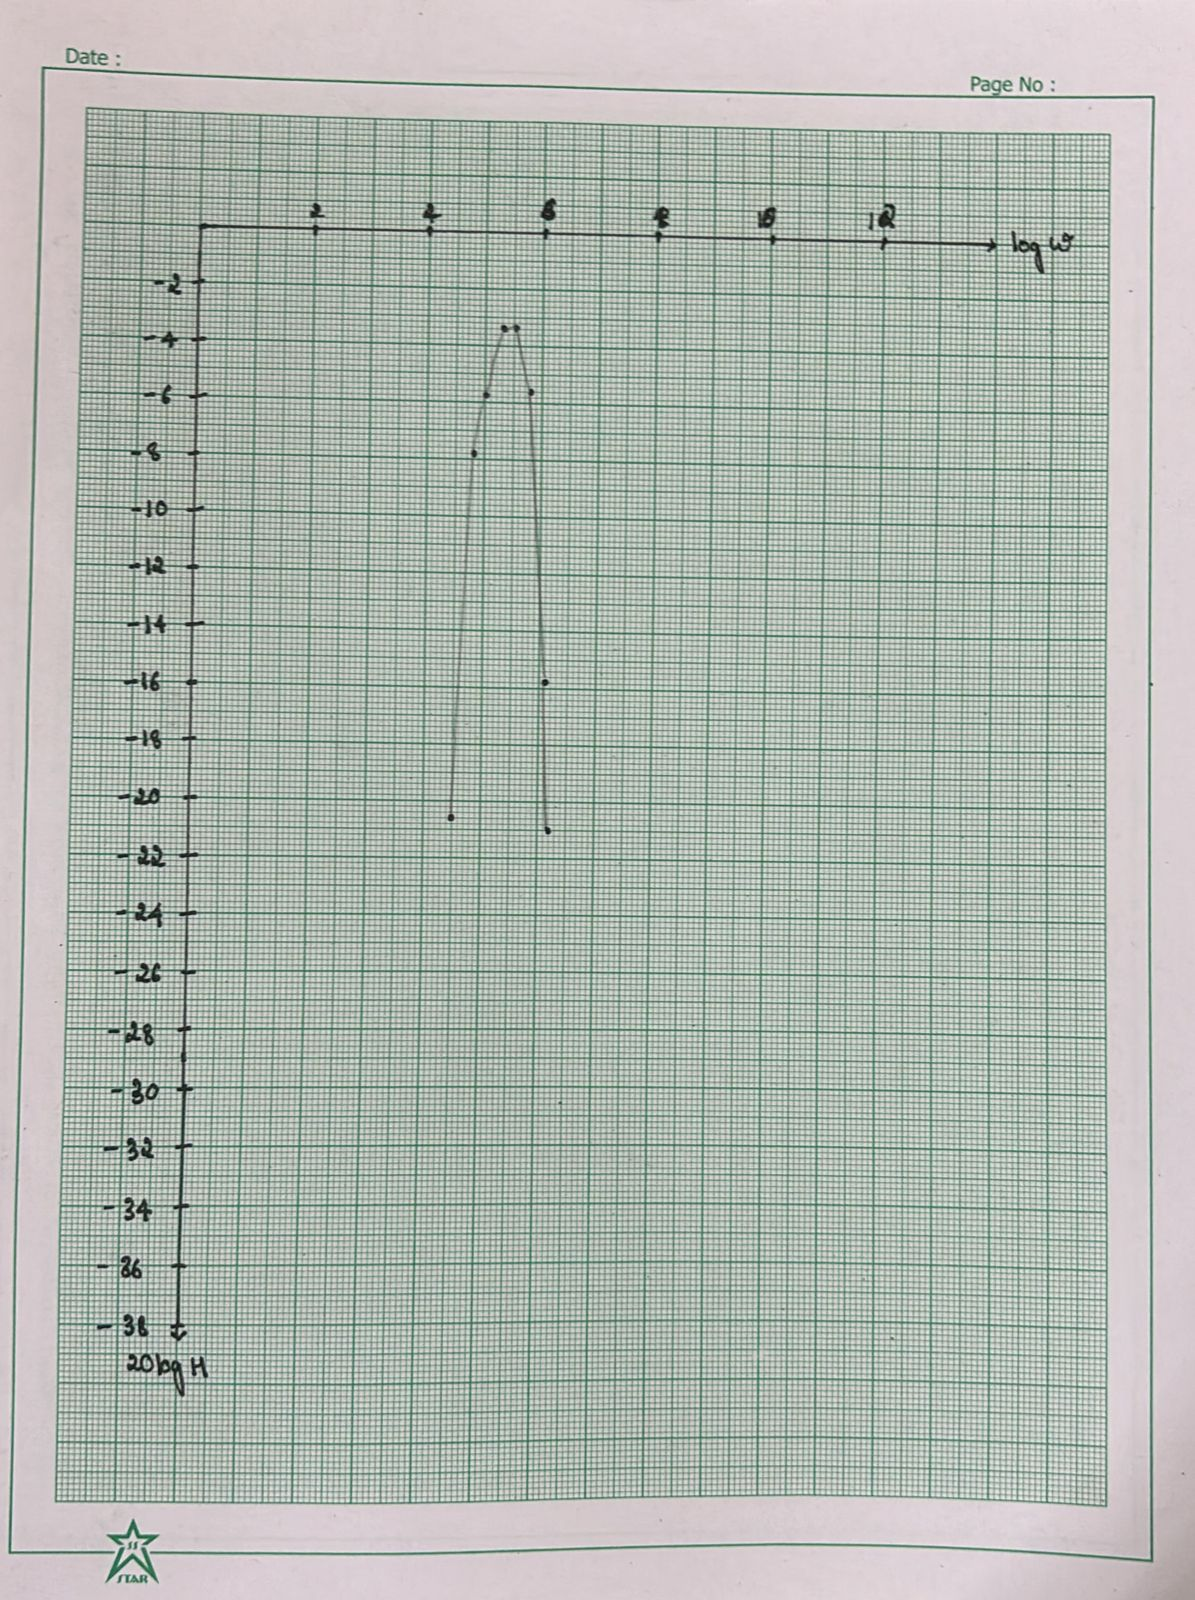
\includegraphics[width=0.5\linewidth]{figs/bandpass_graph.jpeg}
    \caption{Band Pass Filter Graph}
    \label{fig:enter-label}
\end{figure}

Images of oscilloscope while capturing response may be found in the respective folders in the below link, \url{https://github.com/ArjunPavanje/EE1200/tree/main/Experiment_6/figs}


\section*{7 Conclusion}
This experiment demonstrates how Sallen-Key filters can be constructed, and how a high pass and a lowpass filter together can be used to create a bandpass filter.
\end{document}

